\documentclass[12pt,a4paper]{article}
\usepackage[top=25.4mm, bottom=25.4mm, left=19.1mm, right=19.1mm]{geometry}


\usepackage[latin2]{inputenc}
\usepackage{graphicx}
\graphicspath{ {./images/} }
\usepackage{ulem}
\usepackage{amsmath}
\usepackage[document]{ragged2e}

\setlength{\parindent}{4em}
\setlength{\parskip}{1em}
\usepackage{hyperref}

\usepackage{fancyhdr}
\pagestyle{fancy}
\fancyhf{}
\fancyhead[LO]{\textbf{\small IoT and Smart Analytics}\\
\text{\small A Program by IIITH and TalentSprint}}

\usepackage{xcolor}
\usepackage{lipsum}

\rhead{\begin{picture}(0,0) \put(-250,-2){
\includegraphics[width=9cm]{EXP_08_Images/ts-iisc-logo-pr.png}} \end{picture}}
\cfoot{\thepage}


\begin{document}

\begin{center}

\textbf{\large \\EXPERIMENT 19 }\\[6pt]
\text{Star Network using WiFi with ESP32}
\end{center}

\textbf{\large LEARNING OBJECTIVES:}\\[3pt]
At the end of this experiment, participants will be able to:\vspace{-6mm}\begin{enumerate}
 \setlength\itemsep{-0.3em}
\item Understand the Star Network   \\
\item Understand how to implement Star Network using  ESP32
\end{enumerate}

\textbf{\large APPARATUS REQUIRED:}\\
\vspace{-3mm}
\begin{enumerate}
\setlength\itemsep{-0.3em}
\item ESP32 Module-3 pcs
\item Micro USB cable-1pcs
\item Breadboard-2pcs
\item Power Adapter-1pcs
\item DC-DC Voltage Converter Power Supply Module-1cs
\item Jumper wires
\end{enumerate}

\begin{justify}
\textbf{\large THEORY}\\[3pt]
\textbf{Introduction: }The topology of a wireless network is the way network components have been arranged. It describes the physical layout of the devices and the paths they have between them.  A star topology is an architecture where the wireless devices/nodes communicate point-point with the central device/server/sink. Because each device communicates directly with the gateway, a star topology is also sometimes described as a "point-to-point" or “line-of-sight” architecture. These simple, direct wireless connections make star topologies applicable for simple or low-power applications because they can potentially use the least amount of power of all the topologies.

\begin{center} 
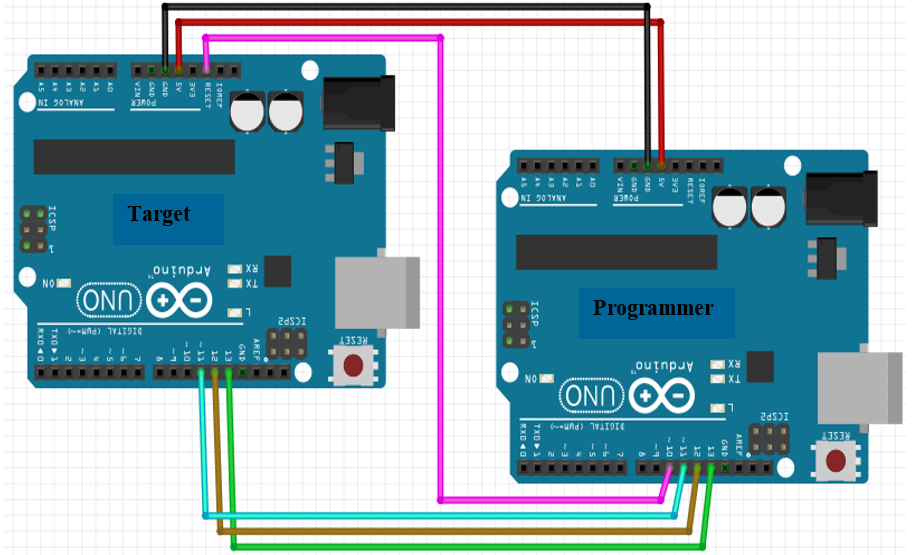
\includegraphics[scale=1]{EXP_19_Images/fig1.png}
\end{center}
\begin{center} {Figure 1.Star Network Topology}\end{center}

\noindent In the case of this experiment, a ESP32 is configured as a softAP and acts as the central device. It also runs a server to handle the requests coming from the clients/slave ESP32s. 

\begin{center} 
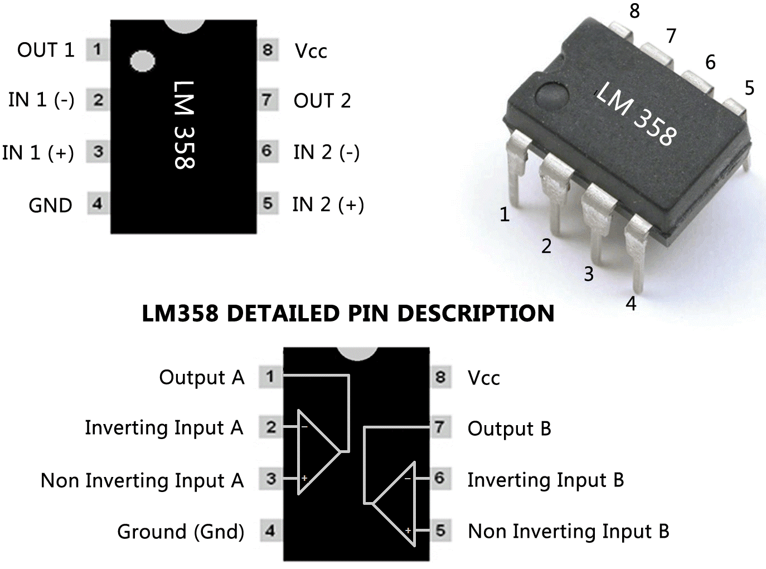
\includegraphics[scale=0.7]{EXP_19_Images/fig2.png}
\end{center}
\begin{center} {Figure 2. ESP32 Master-Slaves}\end{center}\\[21pt]
\noindent \textbf{\large PROCEDURE}\\[3pt]
\textbf{Experiment Overview:}\\
\vspace{-6mm}
\begin{enumerate}
 \setlength\itemsep{-0.3em}
\item Configure a ESP32 which would be the master as Access point with suitable ssid and passowod and obtain its MAC address and IP address. 
\item The master should include the code to handle the incoming requests from the slaves. Have separate code for each slave, as in real scenarios, each slave might have to be handled differently
\item Configure two ESP32s which would be Slave0 and Slave1 as stations and connect to the above given ssid and passoword and to the obtained IP address.
\item The clients should be able to send their names, Slave0 and Slave1 and their corrent status of an LED. The LED can be programmed to be turned on by the command given by the master.
\end{enumerate}
\end{justify}
\vspace{20mm}
\hspace{1cm}\textbf{\large Code for Master:}\\[6pt]


\setlength{\parindent}{5eM}

\#include $<$WiFi.h$>$ //Libraries\\
\#define LED 2 \textcolor{blue}{//Constants}\\
\textcolor{blue}{//Parameters}\\
String nom = "Master";  \\
const char* ssid = "ESP\_Master";\\
const char* password = "password@123";\\
\textcolor{blue}{//Variables}\\
String slaveState = "0";\\
\textcolor{blue}{//Objects}\\
WiFiServer server(80); \\[15pt]

void setup()\\
 \{\\
 \textcolor{blue}{//Init Serial USB}\\
Serial.begin(115200);\\
Serial.println(F("Initialize System"));\\
 \textcolor{blue}{//Init ESP32 Wifi}\\
Serial.println("Configuring access point...");\\
  \textcolor{blue}{// We can remove the password parameter if you want the AP to be open.}\\
WiFi.softAP(ssid, password);\\
IPAddress myIP = WiFi.softAPIP();\\
Serial.print("AP IP address: ");\\
Serial.println(myIP);\\
server.begin();\\
Serial.print(nom);\\
\}\\[15pt]

void loop() \\
\{\\
 clientRequest();\\
\}\\[15pt]

void clientRequest( )  \textcolor{blue}{// function clientRequest}\\
\{\\ 
 \textcolor{blue}{//Check if client connected}\\
 WiFiClient client = server.available();\\
 client.setTimeout(50);\\
 if (client) \\
\{\\
   if (client.connected()) \\
\{\\
    \textcolor{blue}{ //Print client IP address}\\
     Serial.print(":$\rightarrow$");\\
     Serial.println(client.remoteIP());\\
     String request = client.readStringUntil('\textbackslash r');\\ \textcolor{blue}{//receives the message from the client}\\
    
     if (request.indexOf("Slave0") $>= 0$) \\
\{\\
       \textcolor{blue}{//Handle slave request}\\
       Serial.print("From "); \\
       Serial.println(request);\\
       int index = request.indexOf(":");\\
       String slaveid = request.substring(0, index);\\
       slaveState = request.substring(request.indexOf("x") + 1, request.length());\\
       Serial.print("state received: "); \\
       Serial.println(slaveState);\\
       client.print(nom);\\
       client.println(": Hi " + slaveid + "!\textbackslash r'"); \textcolor{blue}{// sends the answer to the client}\\
       client.stop();  \\             \textcolor{blue}{ // terminates the connection with the client}\\
   \}\\ [3pt]
     if (request.indexOf("Slave1")$ >= 0$) \\
 \{\\
      \textcolor{blue}{ //Handle slave request}\\
       Serial.print("From ");\\
       Serial.println(request);\\
       int index = request.indexOf(":");\\
       String slaveid = request.substring(0, index);\\
       slaveState = request.substring(request.indexOf("x") + 1,\\ request.length());\\
       Serial.print("state received: "); \\
       Serial.println(slaveState);\\
       delay(10);\\
       client.print(nom);\\
       client.println(": Hi " + slaveid + "!\textbackslash r'"); \textcolor{blue}{// sends the answer to the client}\\
       client.stop(); \textcolor{blue}{// terminates the connection with the client}\\
    \}\\
   \}\\
 \}\\
\}\\[15pt]
\vspace{5mm}
\setlength{\parindent}{0eM}
\hspace{1cm}\textbf{\large Code for Slave 0:}\\[6pt]
\setlength{\parindent}{5eM}


\#include $<WiFi.h>$  \textcolor{blue}{//Libraries}\\
 \textcolor{blue}{//Constants}\\
\#define LED 2 \\
\#define UPDATE\_TIME 5\\
 \textcolor{blue}{//Parameters}\\
String nom = "Slave0";\\
const char* ssid = "ESP\_Master";\\
const char* password = "password@123";\\
 \textcolor{blue}{//Variables}\\
String command;\\
unsigned long previousRequest = 0;\\
 \textcolor{blue}{//Objects}\\
WiFiClient master;\\
IPAddress server(192,168,4,1);\\[15pt]

void setup()\\
 \{\\
 \textcolor{blue}{//Init Serial USB}\\
 Serial.begin(115200);\\
 Serial.println(F("Initialize System"));\\
 \textcolor{blue}{//Init ESP32 Wifi}\\
 WiFi.begin(ssid, password);\\
while (WiFi.status() != WL\_CONNECTED)\\ 
\{\\
   delay(500);\\
   Serial.print(F("."));\\
 \}\\
 Serial.print(nom);\\
 Serial.print(F(" connected to Wifi! IP address : "));\\
 Serial.println(WiFi.localIP());\\ \textcolor{blue}{// Print the IP address}\\
 pinMode(LED, OUTPUT);\\
 digitalWrite(LED,LOW);\\
\}\\[15pt]

void loop() \\
\{\\
   requestMaster();\\
   delay(2000);\\
\}\\[15pt]

void requestMaster( ) \textcolor{blue}{// function requestMaster }\\
\{\\ \textcolor{blue}{// Request to master}\\
 if ((millis() - previousRequest) $>$ UPDATE\_TIME)\\
\{\\ \textcolor{blue}{// client connect to server every 500ms}\\
   previousRequest = millis();
   if (master.connect(server, 80))\\ 
\{\\\textcolor{blue}{ // Connection to the server}\\
     master.println(nom + ": Hello! my current state is x" +\\ String(digitalRead(LED)) + "\textbackslash r");\\
     \textcolor{blue}{//answer}\\
     String answer = master.readStringUntil('\textbackslash r');   \textcolor{blue}{// receives the answer from the sever}\\
     Serial.println("from " + answer);\\
   \}\\
 \}\\
\}\\
\vspace{10mm}
\setlength{\parindent}{0eM}
\hspace{1cm}\textbf{\large Code for Slave 1:}\\[6pt]
\setlength{\parindent}{5eM}
\#include $<WiFi.h>$  \textcolor{blue}{//Libraries}\\
 \textcolor{blue}{//Constants}\\
\#define LED 2 \\
\#define UPDATE\_TIME 5\\
 \textcolor{blue}{//Parameters}\\
String nom = "Slave1";\\
const char* ssid = "ESP\_Master";\\
const char* password = "password@123";\\
 \textcolor{blue}{//Variables}\\
String command;\\
unsigned long previousRequest = 0;\\
 \textcolor{blue}{//Objects}\\
WiFiClient master;\\
IPAddress server(192,168,4,1);\\[15pt]

void setup()\\
 \{\\
 \textcolor{blue}{//Init Serial USB}\\
 Serial.begin(115200);\\
 Serial.println(F("Initialize System"));\\
 \textcolor{blue}{//Init ESP32 Wifi}\\
 WiFi.begin(ssid, password);\\
while (WiFi.status() != WL\_CONNECTED)\\ 
\{\\
   delay(500);\\
   Serial.print(F("."));\\
 \}\\
 Serial.print(nom);\\
 Serial.print(F(" connected to Wifi! IP address : "));\\
 Serial.println(WiFi.localIP());\\ \textcolor{blue}{// Print the IP address}\\
 pinMode(LED, OUTPUT);\\
 digitalWrite(LED,LOW);\\
\}\\[15pt]

void loop() \\
\{\\
   requestMaster();\\
   delay(2000);\\
\}\\[15pt]

void requestMaster( ) \textcolor{blue}{// function requestMaster }\\
\{\\ \textcolor{blue}{// Request to master}\\
 if ((millis() - previousRequest) $>$ UPDATE\_TIME)\\
\{\\ 
\textcolor{blue}{// client connect to server every 500ms}\\
   previousRequest = millis();\\
   if (master.connect(server, 80))\\ 
\{\\\textcolor{blue}{ // Connection to the server}\\
     master.println(nom + ": Hello! my current state is x" +\\ String(digitalRead(LED)) + "\textbackslash r");\\
     \textcolor{blue}{//answer}\\
     String answer = master.readStringUntil('\textbackslash r');   \textcolor{blue}{// receives the answer from the sever}\\
     Serial.println("from " + answer);\\
   \}\\
 \}\\
\}\\
\vspace{10mm}
\setlength{\parindent}{0eM}
\textbf{\large REFERENCES:}
\vspace{-6mm}
\begin{enumerate}
\setlength\itemsep{-0.3em}
\item  \href {https://www.aranacorp.com/en/communication-between-two-esp32-via-wifi/}{Communication between two ESP32 via WiFi}
\end{enumerate}
\end{document}